\documentclass{beamer}
\usetheme{Boadilla}
\usefonttheme{serif}

%% =========================================================================== %%

\usepackage{amsmath}
\usepackage[makeroom]{cancel}
\usepackage{verbatim}
\usepackage[sort]{natbib}

%% =========================================================================== %%

\title{Gmacs}
\subtitle{BBRKC model comparisons}
\author{The Gmacs Development Team}
%\institute{Quantifish}
\date{\today}

\begin{document}

%% =========================================================================== %%

\begin{frame}
\titlepage
\end{frame}

%% =========================================================================== %%

\begin{frame}
\frametitle{Outline}
\tableofcontents
\end{frame}

%% =========================================================================== %%
%% =========================================================================== %%

\section{Introduction}

%% =========================================================================== %%
%% =========================================================================== %%

\begin{frame}
\frametitle{Introduction}
This presentation provides a comparison between three different Bristol Bay Red
King Crab (BBRKC) stock assessment models. These models inlcude:
\begin{itemize}
\item {\bf OneSex}
\item {\bf TwoSex}
\item {\bf Zheng}~\citep{zheng_bristol_2015}
\end{itemize}
\end{frame}

%% =========================================================================== %%

\subsection{Leading model parameters}
\begin{frame}
\frametitle{Leading model parameters}
\begin{table}
  \centering
  \begin{tabular}{ccl}
  \hline
  Symbol & Support & Description \\
  \hline
      \textcolor{red}{$M_0$} & $0 < \textcolor{red}{M_0} < \infty$ & Initial instantaneous natural mortality rate\\
      \textcolor{red}{$R_0$} & $0 < \textcolor{red}{R_0} < \infty$ & Unfished average recruitment\\
      \textcolor{red}{$\ddot{R}$} & $0 < \textcolor{red}{\ddot{R}} < \infty$ & Initial recruitment\\
      \textcolor{red}{$\bar{R}$} & $0 < \textcolor{red}{\bar{R}} < \infty$ & Average recruitment\\
      \textcolor{red}{$\alpha_r$} & $\textcolor{red}{\alpha_r} > 0$ & Mode of size-at-recruitment\\
      \textcolor{red}{$\beta_r $} & $\textcolor{red}{\beta_r} > 0$ & Shape parameter for size-at-recruitment\\
      \textcolor{red}{$\kappa$} & $\textcolor{red}{\kappa} > 1$ & Recruitment compensation ratio\\
  \hline
  \end{tabular}
\end{table}
We group the leading model parameters into the vector
\begin{equation*}
  \textcolor{red}{\boldsymbol\theta} = \{ \textcolor{red}{M_0},
  \textcolor{red}{R_0}, \textcolor{red}{\ddot{R}}, \textcolor{red}{\bar{R}},
  \textcolor{red}{\alpha_r}, \textcolor{red}{\beta_r}, \textcolor{red}{\kappa} \}.
\end{equation*}
\end{frame}

%% =========================================================================== %%

\subsection{Growth parameters}
\begin{frame}
\frametitle{Growth parameters}
\begin{table}
  \centering
  \begin{tabular}{ccl}
  \hline
  Symbol & Support & Description \\
  \hline
      \textcolor{red}{$\alpha_h$} & $\textcolor{red}{\alpha_h} > 0$ & Mode of size-at-recruitment\\
      \textcolor{red}{$\beta_h$} & $\textcolor{red}{\beta_h} > 0$ & Shape parameter for size-at-recruitment\\
      \textcolor{red}{$\varphi_h$} & $\textcolor{red}{\varphi_h} > 0$ & Instantaneous natural mortality rate\\
      \textcolor{red}{$\mu_h$} & $\textcolor{red}{\mu_h} > 0$ & Length at 50\% molting probability\\
      \textcolor{red}{$c_h$} & $\textcolor{red}{c_h} > 0$ & Coefficient of variation of molting probability\\
  \hline
  \end{tabular}
\end{table}
We group the growth parameters into the vector
\begin{equation*}
  \textcolor{red}{\boldsymbol\psi} = \{ \textcolor{red}{\alpha_h}, 
  \textcolor{red}{\beta_h}, \textcolor{red}{\varphi_h}, \textcolor{red}{\mu_h},
  \textcolor{red}{c_h} \}.
\end{equation*}
\end{frame}

%% =========================================================================== %%

\subsection{Latent states}
\begin{frame}
\frametitle{Latent states}
\begin{table}
  \centering
  \begin{tabular}{ccl}
  \hline
  Symbol & Support & Description \\
  \hline
      \textcolor{red}{$\boldsymbol\nu$} & $\ell \times 1$ & Initial recuitment deviates \\
      \textcolor{red}{$\boldsymbol\xi$} & &  Discard mortality rate\\
  \hline
  \end{tabular}
\end{table}
We group the latent states into the vector
\begin{equation*}
  \textcolor{red}{\boldsymbol\omega} = \{ \textcolor{red}{\boldsymbol\nu},
  \textcolor{red}{\boldsymbol\xi} \}.
\end{equation*}
\end{frame}

%% =========================================================================== %%
%% =========================================================================== %%

\section{Size, weight, molting and growth}

%% =========================================================================== %%
%% =========================================================================== %%

\begin{frame}
\frametitle{Size-weight ($w_{h,\ell}$)}
Mean weight at size ($\ell$) by sex ($h$)
\begin{figure}[!htbp]
  \centering
  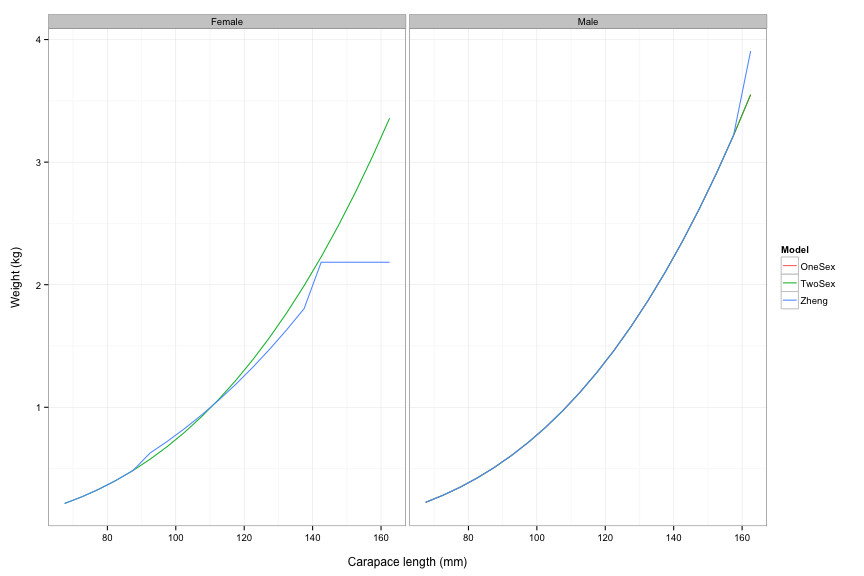
\includegraphics[width=0.75\linewidth]{figure/length_weight-1.png}
\end{figure}
\end{frame}

%% =========================================================================== %%

%\subsection{Maturity ($m_{h,\ell}$)}
%\begin{frame}
%Average proportion mature at length ($\ell$) by sex ($h$)
%\frametitle{Size-weight ($m_{h,\ell}$)}
%\begin{figure}[!htbp]
%  \centering
%  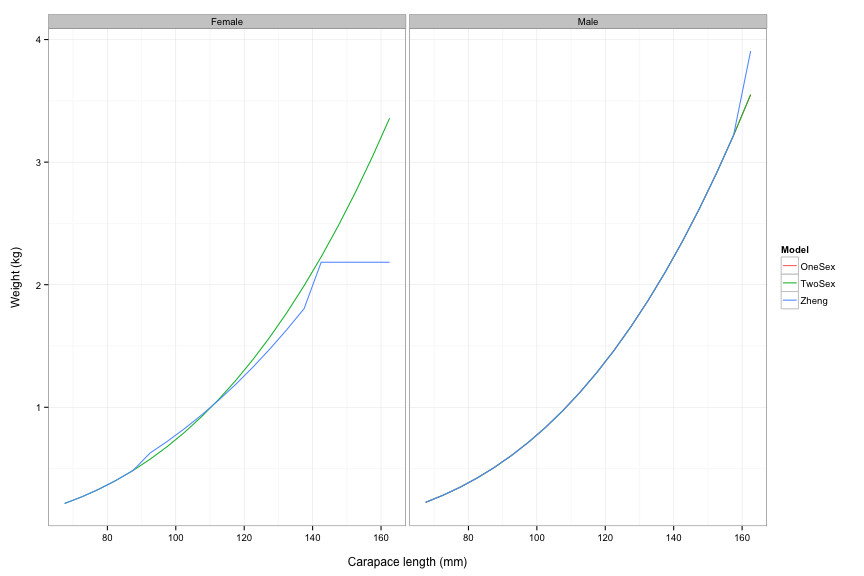
\includegraphics[width=0.75\linewidth]{figure/length_weight-1.png}
%\end{figure}
%\end{frame}

%% =========================================================================== %%

\begin{frame}
\frametitle{Growth increments ($a_{h,\ell}$)}
\begin{figure}[!htbp]
  \centering
  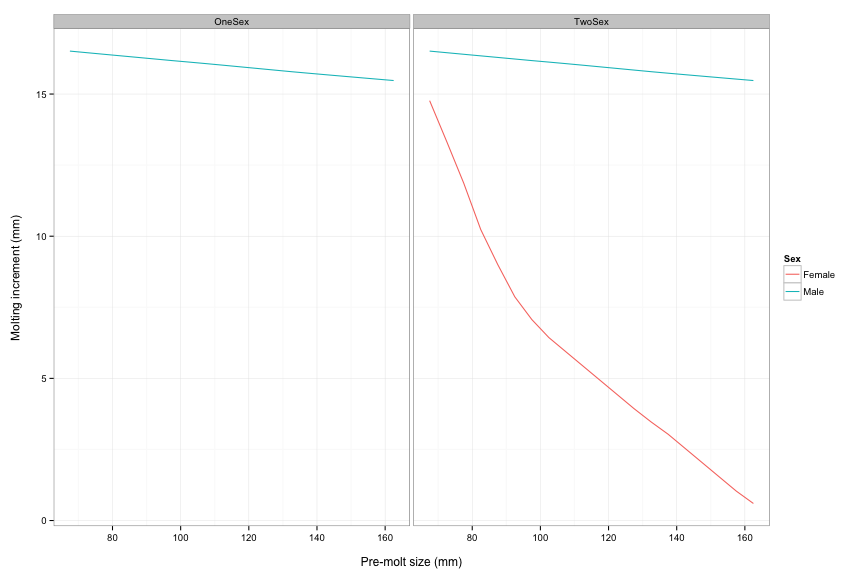
\includegraphics[width=0.75\linewidth]{figure/growth_inc-1.png}
\end{figure}
No comparison with~\citet{zheng_bristol_2015} on plot.
\end{frame}

%% =========================================================================== %%

\begin{frame}
\frametitle{Growth transitions ($\boldsymbol{G}_h$)}
\begin{figure}[!htbp]
  \centering
  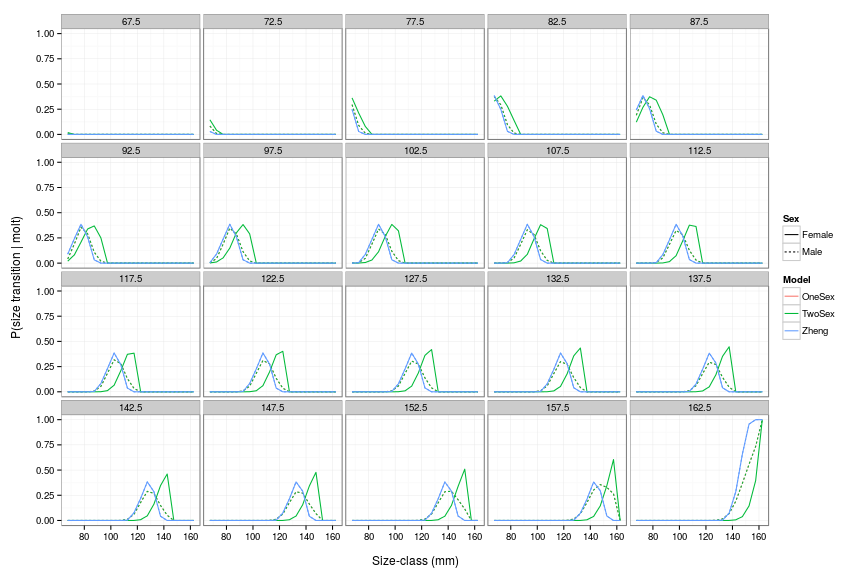
\includegraphics[width=0.75\linewidth]{figure/growth_trans-1.png}
\end{figure}
\end{frame}

%% =========================================================================== %%

\begin{frame}
\frametitle{Molt probability ($\boldsymbol{P}_h$)}
\begin{figure}[!htbp]
  \centering
  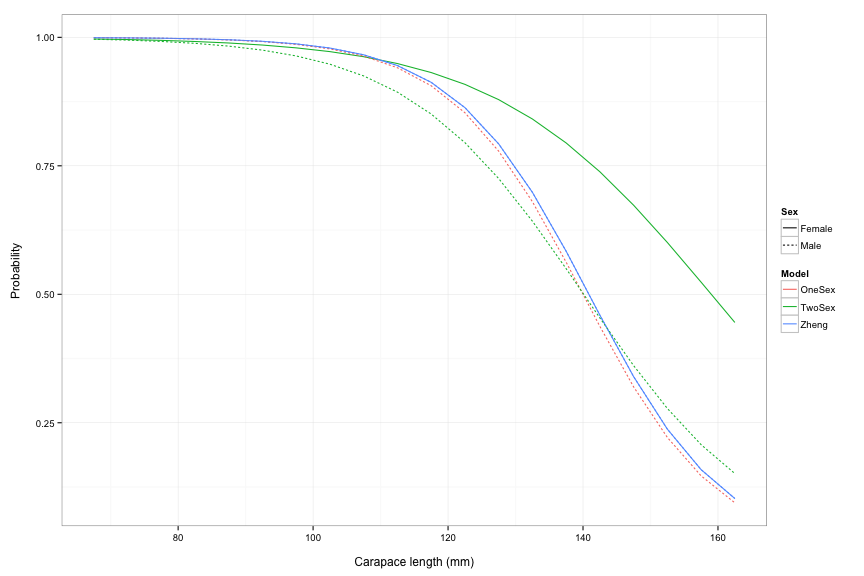
\includegraphics[width=0.75\linewidth]{figure/molt_prob-1.png}
\end{figure}
\end{frame}

%% =========================================================================== %%

\begin{frame}
\frametitle{Size transitions  ($\boldsymbol{P}_h \boldsymbol{G}_h$)}
\begin{figure}[!htbp]
  \centering
  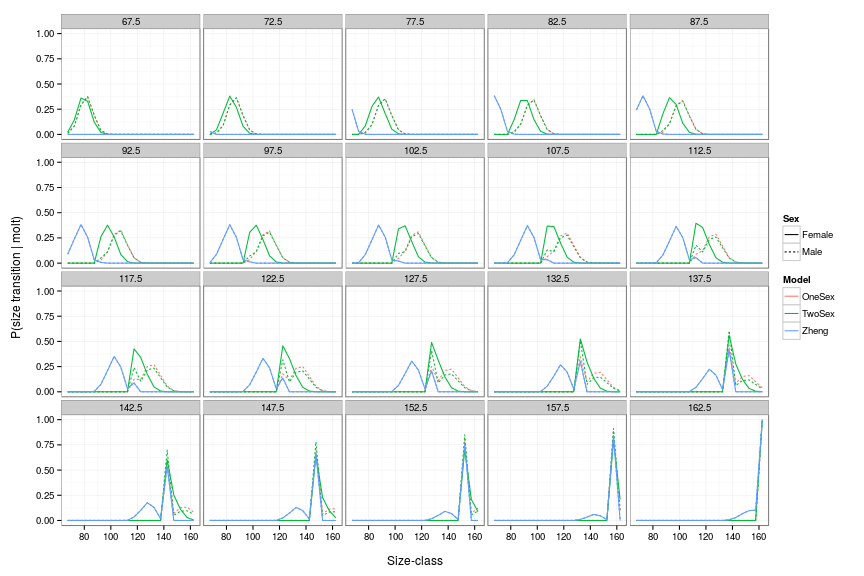
\includegraphics[width=0.75\linewidth]{figure/size_trans-1.png}
\end{figure}
\end{frame}

%% =========================================================================== %%
%% =========================================================================== %%

\section{Natural mortality}

%% =========================================================================== %%
%% =========================================================================== %%

\begin{frame}
\frametitle{Natural mortality}
Time-varying natural mortality is specified using the {\bf blocked changes}
option in Gmacs. The model constrains $M_{h,i}$ by the variance
($\sigma^2_M$). We used the parameters $\sigma^2_M = 0.04$ and four specific
years (1976, 1980, 1985, 1994) we get
\begin{figure}[!htbp]
  \centering
  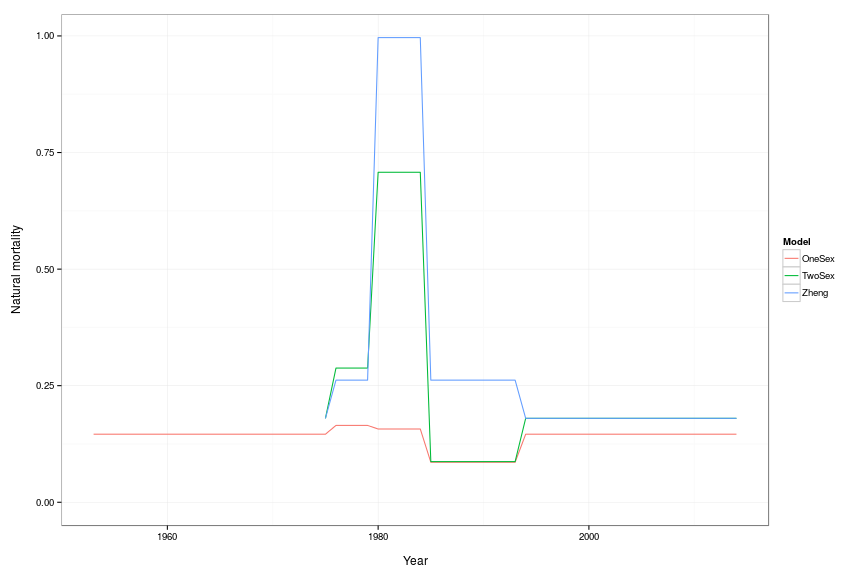
\includegraphics[width=0.65\linewidth]{figure/natural_mortality-1.png}
\end{figure}
\end{frame}

%% =========================================================================== %%
%% =========================================================================== %%

\section{Selectivity, retention, fishing}

%% =========================================================================== %%
%% =========================================================================== %%

\begin{frame}
\frametitle{Selectivity and retention}
Assuming that selectivity for the NMFS trawl fishery is split into two blocks
(1975-1981 and 1982-2014) and that retention is constant with time
$\boldsymbol{y}_{h,i,k} = \boldsymbol{y}_{h,k}$
\begin{figure}[!htbp]
  \centering
  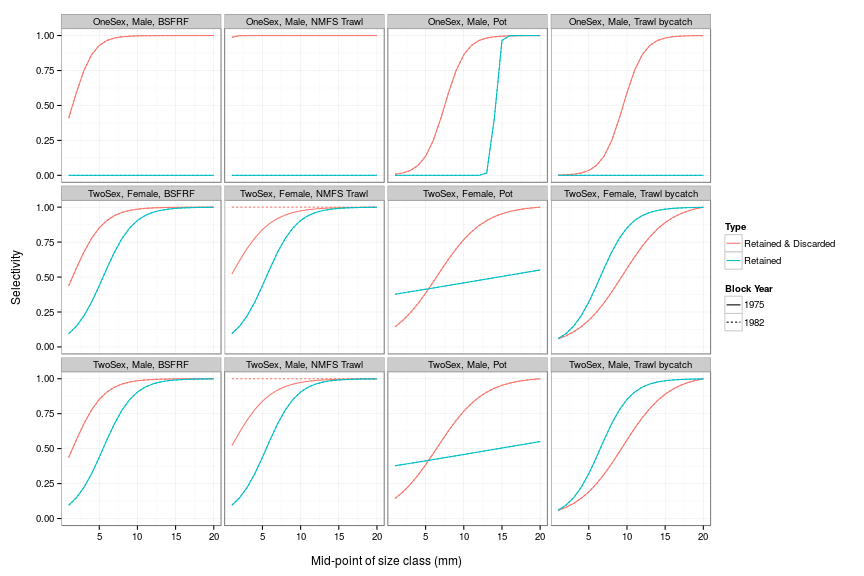
\includegraphics[width=0.6\linewidth]{figure/selectivity-1.png}
\end{figure}
No comparison with~\citet{zheng_bristol_2015} on plot.
\end{frame}

%% =========================================================================== %%

\begin{frame}
\frametitle{Catch}
\begin{figure}[!htbp]
  \centering
  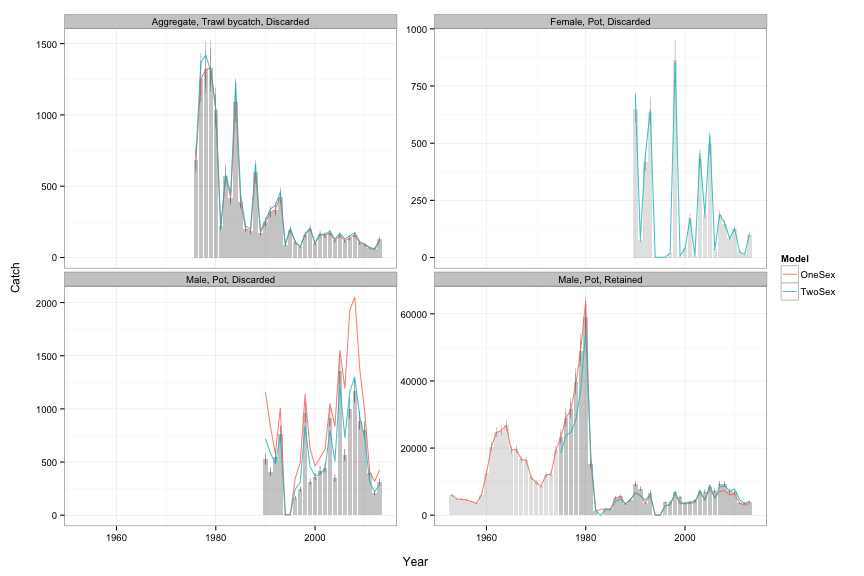
\includegraphics[width=0.6\linewidth]{figure/fit_to_catch-1.png}
\end{figure}
No comparison with~\citet{zheng_bristol_2015} on plot.
\end{frame}

%% =========================================================================== %%
%% =========================================================================== %%

\section{Recruitment}

%% =========================================================================== %%
%% =========================================================================== %%

\begin{frame}
\frametitle{Recruitment}
Recruitment size-distribution
\begin{figure}[!htbp]
  \centering
  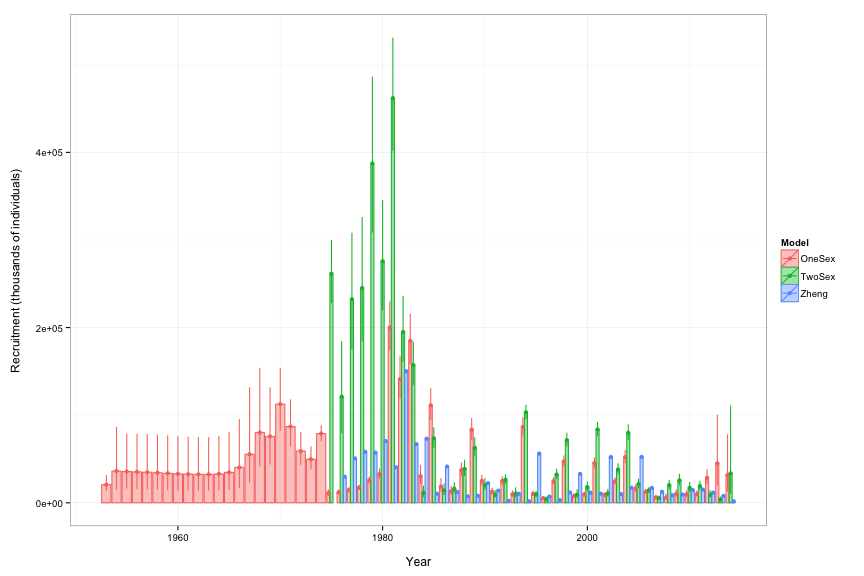
\includegraphics[width=0.6\linewidth]{figure/recruitment-1.png}
\end{figure}
\end{frame}

%% =========================================================================== %%
%% =========================================================================== %%

\section{Initialization}

%% =========================================================================== %%
%% =========================================================================== %%

\begin{frame}
\frametitle{Initial recruitment}
Recruitment size-distribution
\begin{figure}[!htbp]
  \centering
  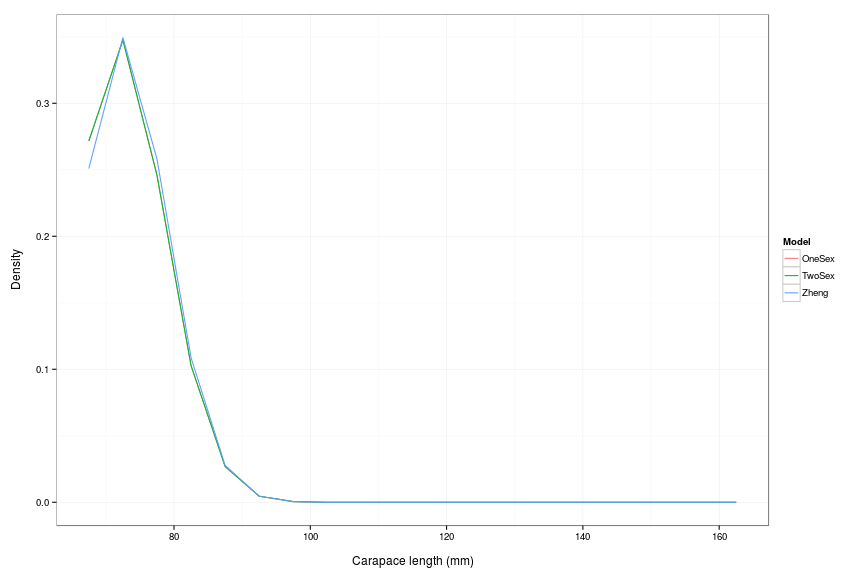
\includegraphics[width=0.6\linewidth]{figure/init_rec-1.png}
\end{figure}
\end{frame}

%% =========================================================================== %%

\begin{frame}
\frametitle{Initial numbers}
\begin{figure}[!htbp]
  \centering
  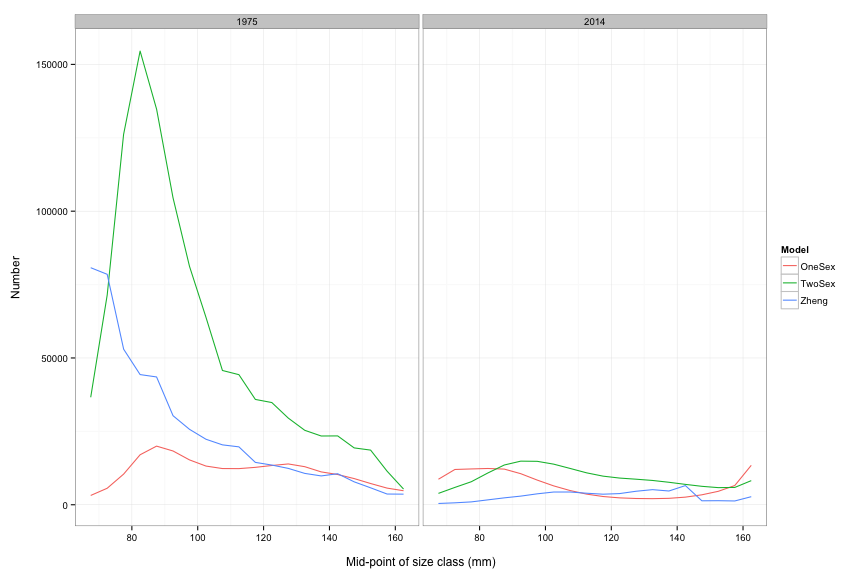
\includegraphics[width=0.6\linewidth]{figure/init_N-1.png}
\end{figure}
\end{frame}

%% =========================================================================== %%
%% =========================================================================== %%

\section{Fits to data}

%% =========================================================================== %%
%% =========================================================================== %%

\subsection{Survey}
\begin{frame}
\frametitle{Survey}
\begin{figure}[!htbp]
  \centering
  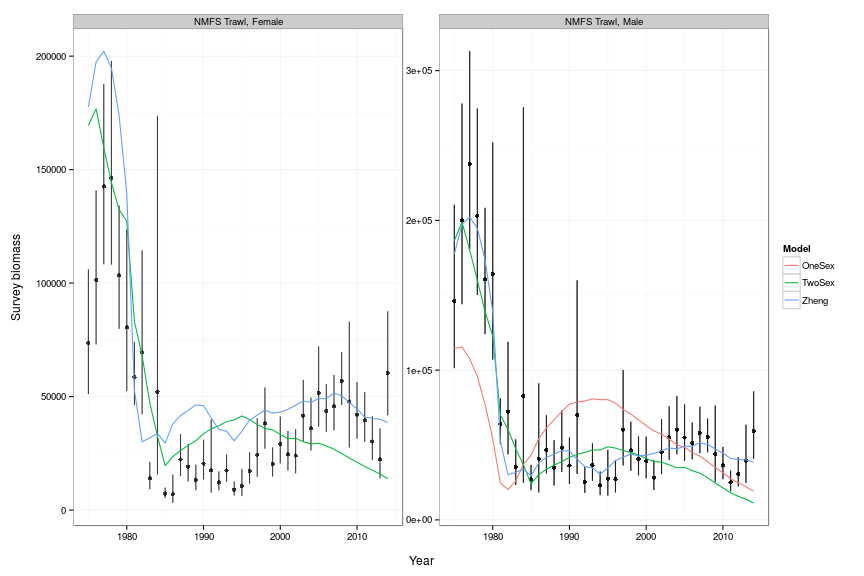
\includegraphics[width=0.6\linewidth]{figure/survey_biomass-1.png}
\end{figure}
\end{frame}

%% =========================================================================== %%

\subsection{Size composition}
\begin{frame}
\frametitle{Size composition}
\begin{figure}[!htbp]
  \centering
  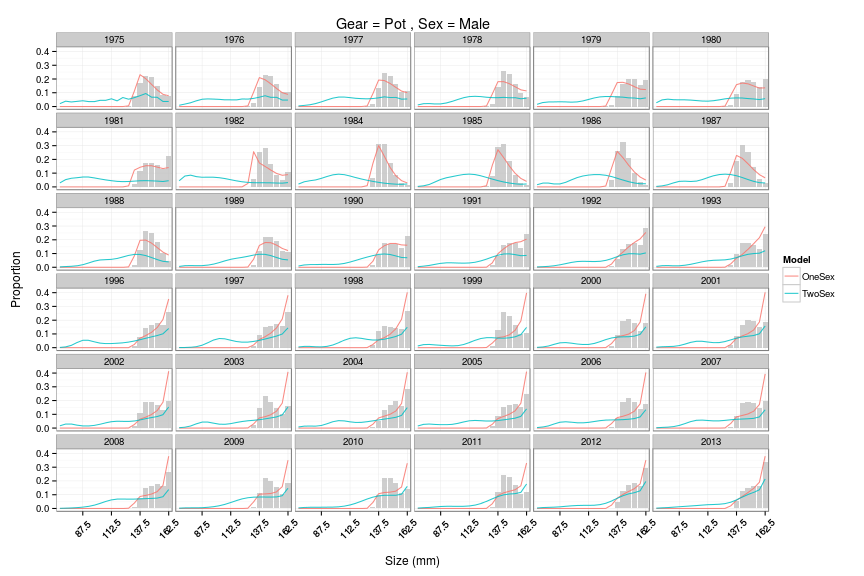
\includegraphics[width=0.6\linewidth]{figure/sc_pot_m-1.png}
\end{figure}
No comparison with~\citet{zheng_bristol_2015} on plot.
\end{frame}

%% =========================================================================== %%
%% =========================================================================== %%

\section{Mature male biomass}

%% =========================================================================== %%
%% =========================================================================== %%

\begin{frame}
\frametitle{Mature male biomass}
\begin{figure}[!htbp]
  \centering
  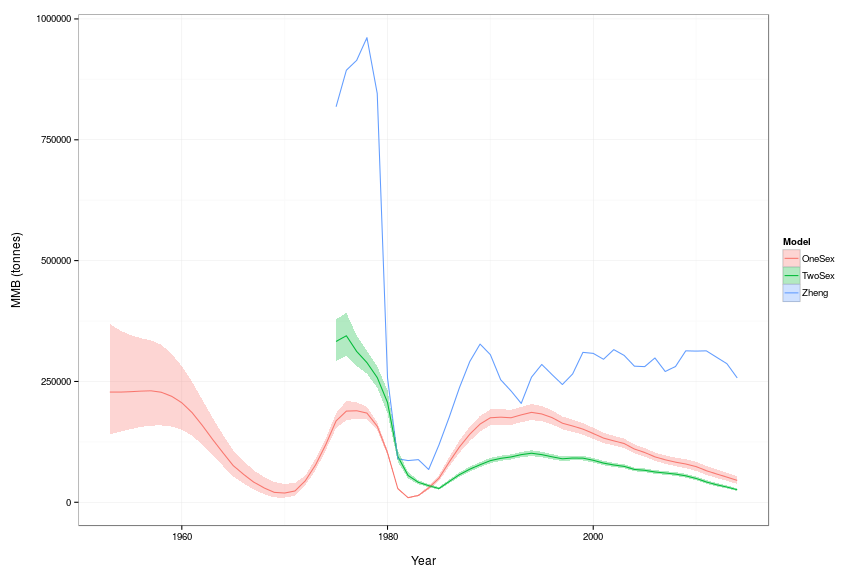
\includegraphics[width=0.6\linewidth]{figure/spawning_stock_biomass-1.png}
\end{figure}
\end{frame}

%% =========================================================================== %%

\begin{frame}
\frametitle{References}
\bibliographystyle{agsm}
\bibliography{../references/Gmacs}
\end{frame}

%% =========================================================================== %%

\end{document}